

\section{Tratamiento de Datos}
\subsection{Introducción}

En este documento se presentan los cálculos realizados a partir de las pruebas de vacío y corto circuito, con el objetivo de determinar los parámetros del circuito equivalente. Los resultados obtenidos se analizan tanto para los lados de alta como de baja tensión.

\subsection{Pruebas de Vacío en Baja Tensión (BT)}

Los datos obtenidos en las pruebas de vacío se encuentran en la siguiente tabla:

\begin{table}[h!]
\centering
\begin{tabular}{|c|c|c|}
\hline
\textbf{Voltaje [V]} & \textbf{Corriente [A]} & \textbf{Potencia [kW]} \\ \hline
220                 & 1.6                    & 0.16                   \\ \hline
\end{tabular}
\caption{Pruebas de vacío en BT.}
\end{table}

Con los datos de la tabla anterior, se realizarán los cálculos necesarios para construir el circuito equivalente. En particular, se analizarán los parámetros magnéticos referidos a los lados de alta y baja tensión.

    

\begin{center}
    $Rm = \frac{V^2}{P} = 302,5~[\Omega]$ \\
    \vspace{0.2cm}
    $S = |V||I| = 352[VA]$\\
    \vspace{0.2cm}
    $Q = \sqrt{S^2 - P^2} = 313.5347[VAR]$ \\
    \vspace{0.2cm}
    $X_m = \frac{V^2}{Q} = 154,3689~[\Omega]$ \\

\end{center}


\subsection{Pruebas de Corto Circuito en Baja Tensión (BT)}

Los datos obtenidos en las pruebas de corto circuito se presentan en la siguiente tabla:

\begin{table}[h!]
\centering
\begin{tabular}{|c|c|c|}
\hline
\textbf{Voltaje [V]} & \textbf{Corriente [A]} & \textbf{Potencia [kW]} \\ \hline
10.06               & 5.42                   & 0.035                  \\ \hline
\end{tabular}
\caption{Pruebas de corto circuito en BT.}
\end{table}

A partir de estos datos, se calcularán las pérdidas de bobinado de cobre. Además, se podrán obtener los parámetros equivalentes referidos al lado de alta tensión.

\begin{center}
    $R_{cc} = \frac{P}{I^2} = 1,1974~[\Omega]$ \\
    \vspace{0.2cm}
    $Z_{cc} = \frac{V}{I} = 1,8561~[\Omega] $ \\
    \vspace{0.2cm}
    $X_{cc} = \sqrt{Z_{cc}^2 - R_{cc}^2} = 1,4232~[\Omega]$ \\
\end{center}


\subsubsection{Modelo del Circuito Equivalente}

En la Figura \ref{fig:modelo_autotransformador} se muestra el modelo del circuito equivalente utilizando un autotransformador.

\begin{figure}[ht!]
    \centering
    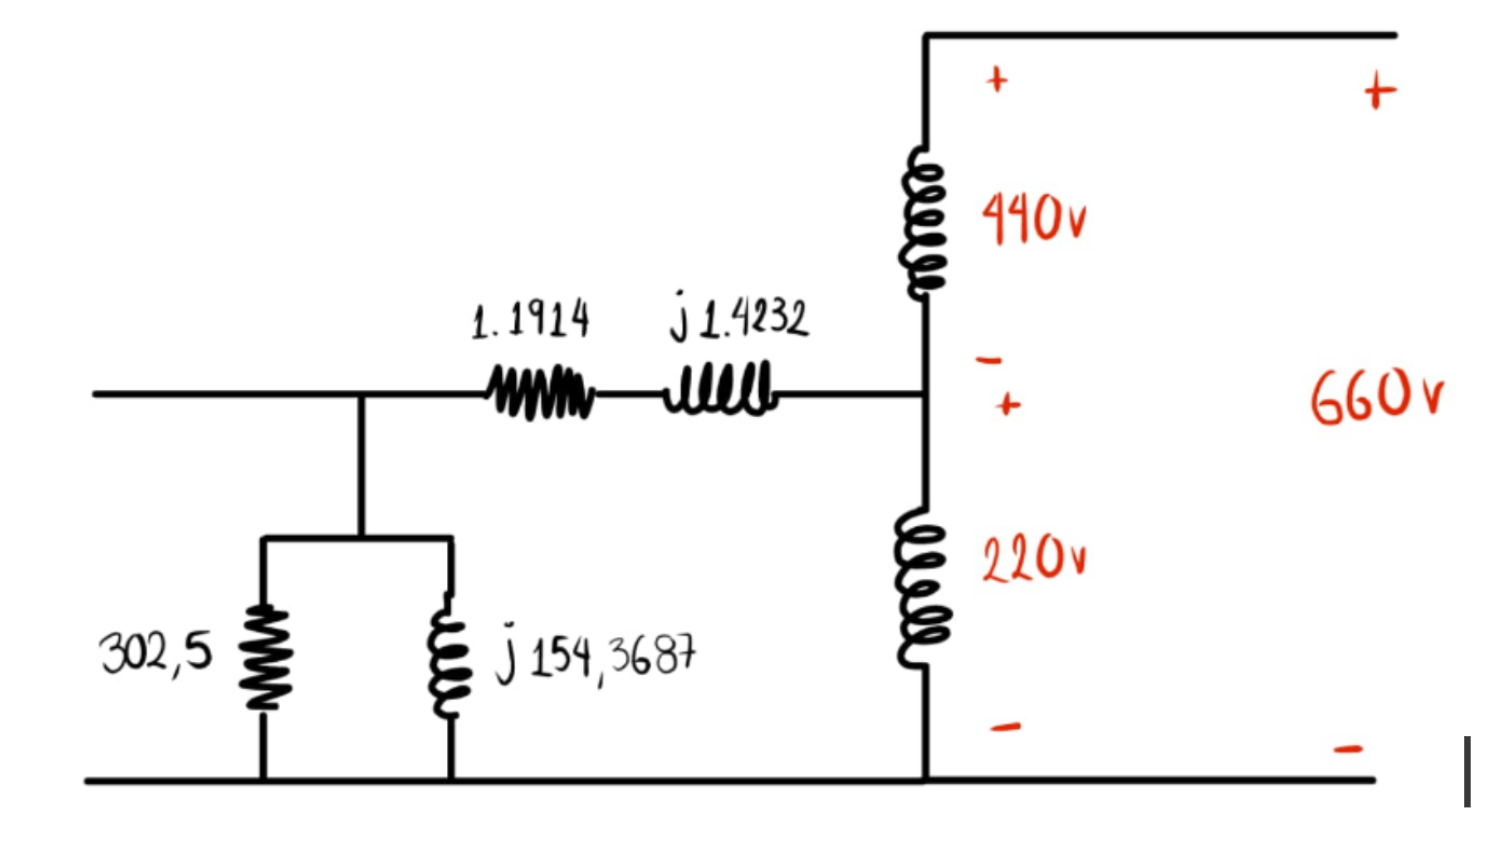
\includegraphics[width=0.48\textwidth]{fot/prac4_regula.png}
    \caption{Modelo del circuito equivalente de un autotransformador.}
    \label{fig:modelo_autotransformador}
\end{figure}


\subsubsection{Eficiencia}

Para los cálculos de eficiencia, se tomaron los valores de potencia de entrada y de salida obtenidos directamente en el laboratorio. A partir de estos datos, se realizó la respectiva operación para determinar la eficiencia del sistema.

\begin{center}
    % Primera ecuación
    $\eta\% = \frac{P_\text{out}}{P_\text{in}} = \frac{0,006}{0,010} * 100 = 60\% \quad \text{Con tensión aplicada: 150,02 V}$ \\
    \vspace{0.5cm}

    % Segunda ecuación
    $\eta\% = \frac{P_\text{out}}{P_\text{in}} = \frac{0,0015}{0,007} * 100 = 21,4286\% \quad \text{Con una tensión aplicada: 133,6 V}$ \\
\end{center}


\subsubsection{Regulación}

Para determinar la regulación se analizaron diferentes tipos de cargas: una \textbf{RL}, una \textbf{RC} y una \textbf{RLC}, todas al mismo nivel de alimentación en el primario. Con estos datos fue posible calcular la regulación de tensión, obteniendo resultados precisos y acordes al sistema estudiado.
\begin{center}
    % Primera ecuación
    $V_{aplicada} = 180,5~\mathrm{V} \quad\Rightarrow\quad V_{sin carga} = 180,5 * \left(\frac{660}{220}\right) = 541,5 \quad \text{Con valores RL} \Rightarrow V = 535~\mathrm{V_{carga}}$ \\
    \vspace{0.5cm}
    % Segunda ecuación
    $\text{Con valores RC} \Rightarrow V = 543~\mathrm{V_{carga}} \quad\Rightarrow\quad \mathrm{VR\%} = \frac{V_\mathrm{fuente} - V_\mathrm{carga}}{V_\mathrm{fuente}} * 100 = \frac{541,5 - 543}{543} * 100 = -0,2762\%$ \\
    \vspace{0.5cm}
    % Tercera ecuación
    $\text{Con valores RLC} \Rightarrow V = 540~\mathrm{V_{carga}} \quad\Rightarrow\quad \mathrm{VR\%} = \frac{V_\mathrm{fuente} - V_\mathrm{carga}}{V_\mathrm{fuente}} * 100 = \frac{541,5 - 540}{540} * 100 = 0,2778\%$ \\
\end{center}